\section{Response Surface Methodology}
\noindent\rule[\linienAbstand]{\linewidth}{\linienDickeDick}

Response surface methodology (RSM) is a statistical technique which is used to model and analyse processes and data in applications in which a response of interest is influenced by several explanatory variables and the aim is to optimise this response.\\
To find the optimum settings of the explanatory variables, it may be useful to proceed in three steps:
\begin{enumerate}
  \item A $2^k$ factorial design (possibly fractional) is used to detect the important influencing factors.
  \item For the most important influencing factors, the main effects are estimated in order to determine the direction of the steepest ascent.
  \item Now we can hope to find the global optimum in the determined direction with a suitabledesign and additional experiments.
\end{enumerate}
This kind of procedure is a response surface exploration which is based on a sequence of experimental design.


\subsection{Response Surface}
\noindent\rule[\linienAbstand]{\linewidth}{\linienDicke}
In the search for relevant influencing factors, we assumed two (or more) levels per factor and used the analysis of variance to estimate and test main effects (and interactions). The model for two factors $A$ and $B$ with two levels each and without interaction is
\begin{equation}
  y_{ij} = \mu_{ij} + \varepsilon_{ij} = \mu + \alpha + \beta_j + \varepsilon_{ij}
\end{equation}

If both explanatory variables $x_1$ and $x_2$ are continuous then the model is
\begin{equation}
  y = f(x_1, x_2) + \varepsilon
\end{equation}
where $\varepsilon$ represents the noise or error observed in the response $y$.
If we denote the expected response by $E(y) = f(x_1, x_2) = \eta$, then the surface represented by
\begin{equation}
  \eta = f(x_1, x_2) + \varepsilon
\end{equation}
is called a response surface.\\

We start with a so-called \textbf{first-order design}, a $2^k$ design with additional measurements in the center of the test conditions.\\
If the response is well modeled by a linear function of the $k$ explanatory variables, the approximating function is the \textbf{first-order model}
\begin{equation}
  y = \beta_0 + \beta_1 x_1 + \beta_2 x_2 + \dots + \beta_k x_k + \varepsilon
\end{equation}

\textbf{Example}\\
A first-order test design and the results of the measurement are reported in the following table.
\begin{table}[H]
  \centering
  \scriptsize
    \begin{tabular}{c|cc|cc|c}
      Run & \multicolumn{2}{c}{Variables in}   & \multicolumn{2}{c}{Variables in} & Yield \\
          & \multicolumn{2}{c}{original units} & \multicolumn{2}{c}{coded untis}  &       \\
          & $T$ [°C] & $t$ [min]               & $\texttt{Temp}$ & $\texttt{Time}$ & y [g]\\ \hline
      1 & 120 & 50 & $-1$ & $-1$ & 52.3 \\
      2 & 160 & 50 & $+1$ & $-1$ & 62.2 \\
      3 & 120 & 70 & $-1$ & $+1$ & 60.1 \\
      4 & 160 & 70 & $+1$ & $+1$ & 70.7 \\ \hline
      5 & 140 & 60 &   0  &   0  & 63.5 \\
      6 & 140 & 60 &   0  &   0  & 63.6
    \end{tabular}
\end{table}
The design is given in coded form and in original units.\\
Now we fit this model to the data of the $2^2$ design with two additional measurements (runs 5 and 6) in the centre of the test conditions.\\
The gradient of the response function
\begin{equation}
  f(\texttt{Temp, Time}) = \beta_0 + \beta_1 \cdot \texttt{Temp} + \beta_2 \cdot \texttt{Time}
\end{equation}
is
\begin{equation}
  \text{grad}\left(f(\texttt{Temp, Time})\right) =
  \begin{pmatrix} \beta_1 \\ \beta_2 \end{pmatrix} =
  \begin{pmatrix} 5.125 \\ 4.075 \end{pmatrix}
\end{equation}
The estimated gradient points into the direction of the largest change in the coded $\texttt{Temp-Time}$-domain. Notice that this direction leads us to a maximal increase of the response.

\begin{figure}[H]
  \centering
  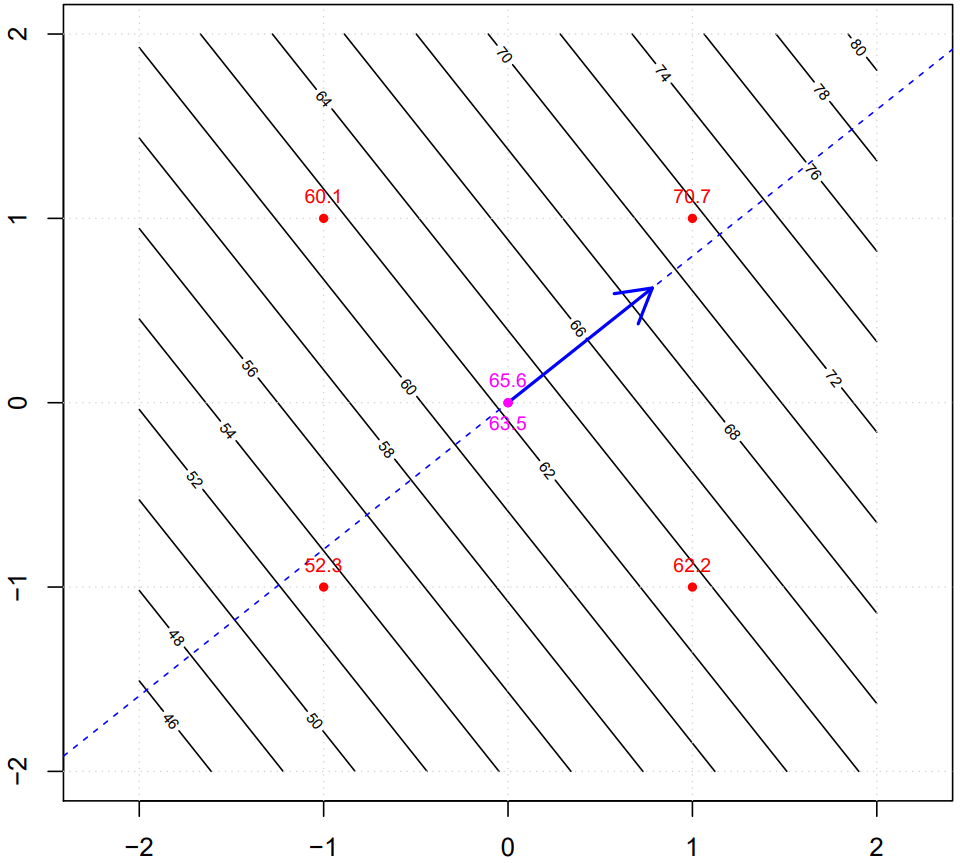
\includegraphics[width=.6\linewidth]{Pics/15.1.2.png}
\end{figure}

There are two reasons why we extended the $2^2$ design with two additional measurements in the centre of the test conditions.
\begin{itemize}
  \item If several measurements for that point are made, then the measurement error can be determined without assuming that the first-order linear model approximates the true response sufficiently well.
  \item It is possible to detect deviations (curvature) from the first-order linear model. If no curvature is present and if the plane is a sufficient approximation of the response within the experimental domain, then the mean of the central observations $\bar{y}_c$ and the mean of all the other observations in the $2^k$ factorial design $\bar{y}_f$ are almost the same. If, on the other hand, this difference is significantly different from zero then this is an indication that a model with curvature is more appropriate.\\
\end{itemize}

The corresponding hypothesis to test the presence of curvature in a $2^k$ design are
\begin{equation}
  \begin{split}
    H_0 &: \;\text{no curvature in the data},\\
    H_1 &: \;\text{curvature in the data}.
  \end{split}
\end{equation}

The test statistic for the curvature in a $2^k$ factorial design is
\begin{equation}
  t_{\text{curve}} = \frac{\bar{y}_c -\bar{y}_f}{\sqrt{s_c^2 \left(\frac{1}{n_c} + \frac{1}{2^k}\right)}}
\end{equation}
Where $s_c^2$ is the empirical variance.
Under the null hypothesis the test statistic $t_{curv}$ follows a $t$-distribution with $n_c - 1$ degrees of freedom.\\

If the first-order linear model is fits the data well then we can search an optimum along the straight line through the centre of the design and along the estimated gradient.

\subsection{Second-Order Response Surface with Interactions}
\noindent\rule[\linienAbstand]{\linewidth}{\linienDicke}
There are two reasons to use a second-order polynomial:\\
\begin{itemize}
  \item If we are close to the optimum and the estimated response plane is almost horizontal, i.e. the estimated coefficients are almost zero.\\
  \item If there is curvature in the system, then a polynomial of higher degree must be used, such as the second-order model
\end{itemize}
\begin{equation}
  y = \beta_0 + \sum_{i=1}^k \beta_i x_i + \sum_{i=1}^k \beta_{ii} x_i^2 + \sum_{i<j} \beta_{ij} x_i x_j + \varepsilon
\end{equation}
In the case of two explanatory variables the model simplifies to
\begin{equation}
  y = \beta_0 + \beta_1 x_1 + \beta_2 x_2 + \beta_{11} x_{1}^2 + \beta_{22}x_{2}^2 + \beta_{12} x_1 x_2 + \varepsilon
\end{equation}

The $2^k$ design is not enough to estimate the parameters in the second-order model. To keep the effort within limits, so-called \emph{rotatable central composite design} or \emph{second-order central composite design} are used. This design can be obtained from a $2^k$ design by adding more experimental conditions.\\
For the case of two explanatory variables all experimental conditions in coded variables (except the centre) are equidistant from the center $(0, 0)$. Each factor is measured at five levels. $(\pm 1, \pm \sqrt{2}, 0)$\\

\textbf{Example (continuation)}\\
The second-order test plan and the results of the measurements are reported in the following table.
\begin{table}[H]
  \centering
  \scriptsize
    \begin{tabular}{c|cc|cc|c}
      Run & \multicolumn{2}{c}{Variables in}   & \multicolumn{2}{c}{Variables in} & Yield \\
          & \multicolumn{2}{c}{original units} & \multicolumn{2}{c}{coded untis}  &       \\
          & $T$ [°C] & $t$ [min]               & $\texttt{Temp}$ & $\texttt{Time}$ & y [g]\\ \hline
      12 & 195 & 80  & $-1$        & $-1$        & 78.7 \\
      13 & 235 & 80  & $+1$        & $-1$        & 76.2 \\
      14 & 195 & 100 & $-1$        & $+1$        & 72.6 \\
      15 & 235 & 100 & $+1$        & $+1$        & 75.5 \\
      16 & 187 & 90  & $-\sqrt{2}$ & 0           & 74.5 \\
      17 & 243 & 90  & $ \sqrt{2}$ & 0           & 76.2 \\
      18 & 215 & 76  & 0           & $-\sqrt{2}$ & 77.8 \\
      19 & 215 & 104 & 0           & $ \sqrt{2}$ & 72.2 \\
      20 & 215 & 90  & 0           & 0           & 80.7
    \end{tabular}
\end{table}
The second-order linear model in original variables is
\begin{equation}
  y = \beta_0 + \beta_1 T + \beta_2 t + \beta_{11} T^2 + \beta_{22}t^2 + \beta_{12}T\cdot t + \varepsilon
\end{equation}
Now we fit this model with the interaction term to the data in original units of the rotatable central composite design and get the estimated second-order response function.

\begin{figure}[H]
  \centering
  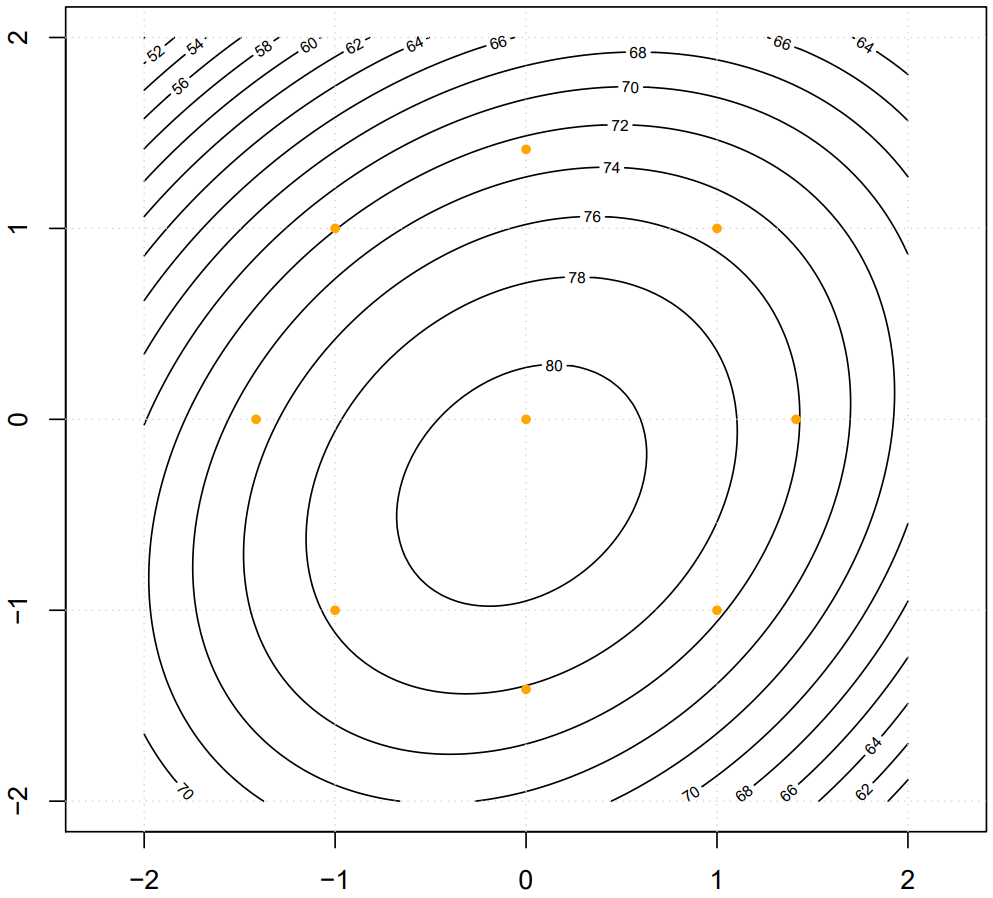
\includegraphics[width=.6\linewidth]{Pics/15.2.1.png}
\end{figure}

A second-order response surface can describe different types of surfaces depending on its parameters.
\begin{itemize}
  \item The surfaces with maximum (or minimum) hardly require any explanation: leaving the optimum in any direction decreases (or increases) the yield $y$.
  \item In the saddle, the yield y may increase or decrease depending on the direction in which the experimental conditions are moving. A fitted saddle is useless to find an optimum.
\end{itemize}

The optimum of the response function can be calculated analytically. The stationary point can be found by setting all $k$ partial derivatives equal to zero.
In the case of two explanatory variables we obtain
\begin{equation}
  \begin{split}
    \frac{\partial}{\partial x_1}f(x_1, x_2) &= \beta_1 + 2\beta_{11} x_1 +  \beta_{12} x_2 = 0 \\
    \frac{\partial}{\partial x_2}f(x_1, x_2) &= \beta_2 +  \beta_{12} x_1 + 2\beta_{22} x_2 = 0
  \end{split}
\end{equation}
and the estimated stationary point is
\begin{equation}
  \hat{x}_1 = \frac{\hat{\beta}_{12} \hat{\beta}_{2} - 2\hat{\beta}_{22} \hat{\beta}_{1}}{4\hat{\beta}_{11} \hat{\beta}_{22} - \hat{\beta}_{12}^2}
  \;\;\;\;\text{and}\;\;\;\;
  \hat{x}_2 = \frac{\hat{\beta}_{12} \hat{\beta}_{1} - 2\hat{\beta}_{11} \hat{\beta}_{2}}{4\hat{\beta}_{11} \hat{\beta}_{22} - \hat{\beta}_{12}^2}
\end{equation}
If the estimated determinant of the Hessian matrix is
\begin{equation}
  4\hat{\beta}_{11} \hat{\beta}_{22} - \hat{\beta}_{12}^2 > 0
\end{equation}
then we have a maximum (or a minimum) otherwise a useless saddle point.\\

\textbf{Summary Response Surface Methodology}\\
\begin{enumerate}
  \item  If the actual settings are far away from the optimum then use a first-order response surface on a $2^k$ fractional factorial design to obtain an overview of the situation.
  \item  Use the method of steepest ascent to obtain further measurements along the gradient till the response gets smaller (larger) again.
  \item  Repeat Step 1 and 2, if necessary, in a vicinity of the optimum found in Step 2.
  \item  Use a rotatable central composite design in the vicinity of the optimum found in Step 3. Estimate the second-order response surface. Find analytically an estimate of the stationary point.
\end{enumerate}

\textbf{All experiments in one plot}\\
\begin{figure}[H]
  \centering
  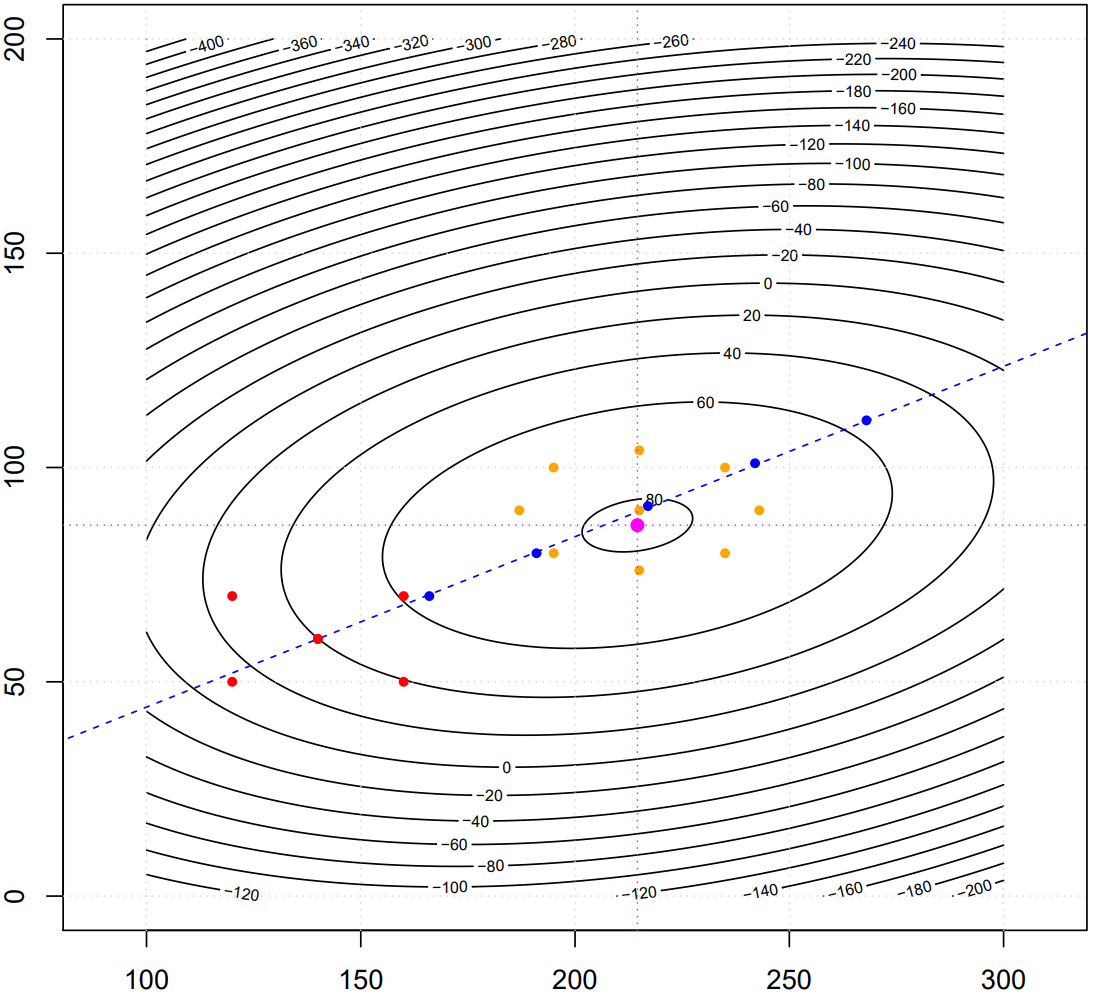
\includegraphics[width=.6\linewidth]{Pics/15.2.3.png}
\end{figure}
Contour plot in original units of the estimated second-order response surface with measurements of the three experiments: Experiment 1 is a $2^2$ factorial design with additional doubled measurement in the centre (red), experiment 2 is an optimisation along the gradient (blue) and experiment 3 is a rotatable central composite design (orange). Optimal settings (magenta).


\newpage
